% Created by tikzDevice version 0.12 on 2019-06-13 00:24:32
% !TEX encoding = UTF-8 Unicode
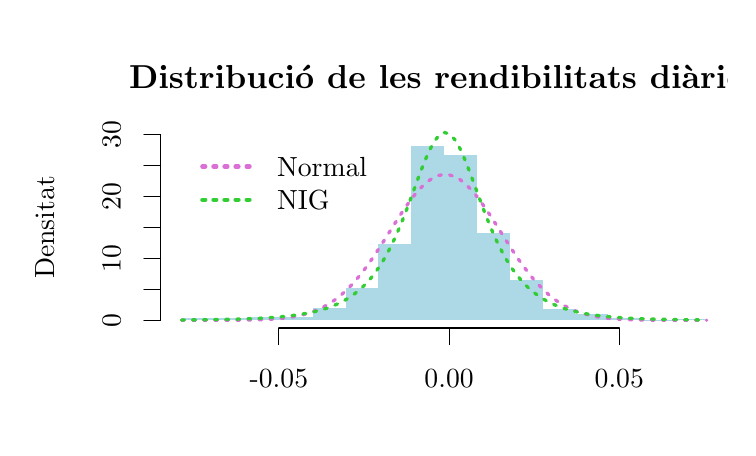
\begin{tikzpicture}[x=1pt,y=1pt]
\definecolor{fillColor}{RGB}{255,255,255}
\path[use as bounding box,fill=fillColor,fill opacity=0.00] (0,0) rectangle (252.94,144.54);
\begin{scope}
\path[clip] ( 48.00, 36.00) rectangle (252.94, 36.13);
\definecolor{fillColor}{RGB}{173,216,230}

\path[fill=fillColor] (142.38, 36.04) --
	(142.38, 36.09) --
	(163.94, 36.09) --
	(163.94, 36.04) --
	cycle;
\definecolor{drawColor}{RGB}{0,0,0}

\path[draw=drawColor,line width= 0.4pt,line join=round] (152.60, 36.04) -- (152.60, 36.09);

\path[draw=drawColor,line width= 0.4pt,dash pattern=on 4pt off 4pt ,line join=round,line cap=round] (110.55, 36.07) -- (142.38, 36.07);

\path[draw=drawColor,line width= 0.4pt,dash pattern=on 4pt off 4pt ,line join=round,line cap=round] (195.67, 36.07) -- (163.94, 36.07);

\path[draw=drawColor,line width= 0.4pt,line join=round,line cap=round] (110.55, 36.05) -- (110.55, 36.08);

\path[draw=drawColor,line width= 0.4pt,line join=round,line cap=round] (195.67, 36.05) -- (195.67, 36.08);
\definecolor{drawColor}{RGB}{255,255,255}

\path[draw=drawColor,line width= 0.4pt,line join=round,line cap=round] (142.38, 36.04) --
	(142.38, 36.09) --
	(163.94, 36.09) --
	(163.94, 36.04) --
	(142.38, 36.04);

\path[draw=drawColor,line width= 0.4pt,line join=round,line cap=round] ( 85.57, 36.07) circle (  2.25);

\path[draw=drawColor,line width= 0.4pt,line join=round,line cap=round] ( 60.58, 36.07) circle (  2.25);

\path[draw=drawColor,line width= 0.4pt,line join=round,line cap=round] (198.27, 36.07) circle (  2.25);

\path[draw=drawColor,line width= 0.4pt,line join=round,line cap=round] (196.62, 36.07) circle (  2.25);

\path[draw=drawColor,line width= 0.4pt,line join=round,line cap=round] (107.04, 36.07) circle (  2.25);

\path[draw=drawColor,line width= 0.4pt,line join=round,line cap=round] (197.12, 36.07) circle (  2.25);

\path[draw=drawColor,line width= 0.4pt,line join=round,line cap=round] ( 72.66, 36.07) circle (  2.25);

\path[draw=drawColor,line width= 0.4pt,line join=round,line cap=round] (215.76, 36.07) circle (  2.25);

\path[draw=drawColor,line width= 0.4pt,line join=round,line cap=round] ( 95.39, 36.07) circle (  2.25);

\path[draw=drawColor,line width= 0.4pt,line join=round,line cap=round] ( 99.96, 36.07) circle (  2.25);

\path[draw=drawColor,line width= 0.4pt,line join=round,line cap=round] (210.64, 36.07) circle (  2.25);

\path[draw=drawColor,line width= 0.4pt,line join=round,line cap=round] (109.18, 36.07) circle (  2.25);

\path[draw=drawColor,line width= 0.4pt,line join=round,line cap=round] (103.93, 36.07) circle (  2.25);

\path[draw=drawColor,line width= 0.4pt,line join=round,line cap=round] ( 88.74, 36.07) circle (  2.25);

\path[draw=drawColor,line width= 0.4pt,line join=round,line cap=round] (209.15, 36.07) circle (  2.25);

\path[draw=drawColor,line width= 0.4pt,line join=round,line cap=round] (203.89, 36.07) circle (  2.25);

\path[draw=drawColor,line width= 0.4pt,line join=round,line cap=round] (203.49, 36.07) circle (  2.25);

\path[draw=drawColor,line width= 0.4pt,line join=round,line cap=round] (101.22, 36.07) circle (  2.25);

\path[draw=drawColor,line width= 0.4pt,line join=round,line cap=round] (200.30, 36.07) circle (  2.25);

\path[draw=drawColor,line width= 0.4pt,line join=round,line cap=round] (108.24, 36.07) circle (  2.25);

\path[draw=drawColor,line width= 0.4pt,line join=round,line cap=round] ( 67.83, 36.07) circle (  2.25);

\path[draw=drawColor,line width= 0.4pt,line join=round,line cap=round] (214.16, 36.07) circle (  2.25);

\path[draw=drawColor,line width= 0.4pt,line join=round,line cap=round] (206.14, 36.07) circle (  2.25);

\path[draw=drawColor,line width= 0.4pt,line join=round,line cap=round] (243.51, 36.07) circle (  2.25);

\path[draw=drawColor,line width= 0.4pt,line join=round,line cap=round] ( 98.46, 36.07) circle (  2.25);

\path[draw=drawColor,line width= 0.4pt,line join=round,line cap=round] (245.35, 36.07) circle (  2.25);

\path[draw=drawColor,line width= 0.4pt,line join=round,line cap=round] (222.55, 36.07) circle (  2.25);

\path[draw=drawColor,line width= 0.4pt,line join=round,line cap=round] (212.08, 36.07) circle (  2.25);

\path[draw=drawColor,line width= 0.4pt,line join=round,line cap=round] (101.17, 36.07) circle (  2.25);

\path[draw=drawColor,line width= 0.4pt,line join=round,line cap=round] ( 83.86, 36.07) circle (  2.25);

\path[draw=drawColor,line width= 0.4pt,line join=round,line cap=round] (100.64, 36.07) circle (  2.25);

\path[draw=drawColor,line width= 0.4pt,line join=round,line cap=round] ( 79.93, 36.07) circle (  2.25);

\path[draw=drawColor,line width= 0.4pt,line join=round,line cap=round] (108.84, 36.07) circle (  2.25);

\path[draw=drawColor,line width= 0.4pt,line join=round,line cap=round] ( 73.53, 36.07) circle (  2.25);

\path[draw=drawColor,line width= 0.4pt,line join=round,line cap=round] (106.94, 36.07) circle (  2.25);

\path[draw=drawColor,line width= 0.4pt,line join=round,line cap=round] (201.77, 36.07) circle (  2.25);

\path[draw=drawColor,line width= 0.4pt,line join=round,line cap=round] (106.44, 36.07) circle (  2.25);

\path[draw=drawColor,line width= 0.4pt,line join=round,line cap=round] (104.11, 36.07) circle (  2.25);

\path[draw=drawColor,line width= 0.4pt,line join=round,line cap=round] (103.10, 36.07) circle (  2.25);

\path[draw=drawColor,line width= 0.4pt,line join=round,line cap=round] ( 55.59, 36.07) circle (  2.25);

\path[draw=drawColor,line width= 0.4pt,line join=round,line cap=round] ( 81.64, 36.07) circle (  2.25);

\path[draw=drawColor,line width= 0.4pt,line join=round,line cap=round] (205.97, 36.07) circle (  2.25);

\path[draw=drawColor,line width= 0.4pt,line join=round,line cap=round] (109.61, 36.07) circle (  2.25);

\path[draw=drawColor,line width= 0.4pt,line join=round,line cap=round] (211.73, 36.07) circle (  2.25);

\path[draw=drawColor,line width= 0.4pt,line join=round,line cap=round] (202.61, 36.07) circle (  2.25);

\path[draw=drawColor,line width= 0.4pt,line join=round,line cap=round] ( 63.93, 36.07) circle (  2.25);

\path[draw=drawColor,line width= 0.4pt,line join=round,line cap=round] (105.20, 36.07) circle (  2.25);

\path[draw=drawColor,line width= 0.4pt,line join=round,line cap=round] (231.79, 36.07) circle (  2.25);
\end{scope}
\begin{scope}
\path[clip] (  0.00,  0.00) rectangle (252.94,144.54);
\definecolor{drawColor}{RGB}{0,0,0}

\path[draw=drawColor,line width= 0.4pt,line join=round,line cap=round] ( 90.78, 36.00) -- (213.78, 36.00);

\path[draw=drawColor,line width= 0.4pt,line join=round,line cap=round] ( 90.78, 36.00) -- ( 90.78, 30.00);

\path[draw=drawColor,line width= 0.4pt,line join=round,line cap=round] (152.28, 36.00) -- (152.28, 30.00);

\path[draw=drawColor,line width= 0.4pt,line join=round,line cap=round] (213.78, 36.00) -- (213.78, 30.00);

\node[text=drawColor,anchor=base,inner sep=0pt, outer sep=0pt, scale=  1.00] at ( 90.78, 14.40) {-0.05};

\node[text=drawColor,anchor=base,inner sep=0pt, outer sep=0pt, scale=  1.00] at (152.28, 14.40) {0.00};

\node[text=drawColor,anchor=base,inner sep=0pt, outer sep=0pt, scale=  1.00] at (213.78, 14.40) {0.05};
\end{scope}
\begin{scope}
\path[clip] (  0.00, 36.13) rectangle (252.94,144.54);
\definecolor{drawColor}{RGB}{0,0,0}

\node[text=drawColor,anchor=base,inner sep=0pt, outer sep=0pt, scale=  1.20] at (150.47,122.40) {\bfseries Distribució de les rendibilitats diàries};

\node[text=drawColor,rotate= 90.00,anchor=base,inner sep=0pt, outer sep=0pt, scale=  1.00] at (  9.60, 72.34) {Densitat};
\end{scope}
\begin{scope}
\path[clip] (  0.00,  0.00) rectangle (252.94,144.54);
\definecolor{drawColor}{RGB}{0,0,0}

\path[draw=drawColor,line width= 0.4pt,line join=round,line cap=round] ( 48.00, 38.82) -- ( 48.00,105.86);

\path[draw=drawColor,line width= 0.4pt,line join=round,line cap=round] ( 48.00, 38.82) -- ( 42.00, 38.82);

\path[draw=drawColor,line width= 0.4pt,line join=round,line cap=round] ( 48.00, 49.99) -- ( 42.00, 49.99);

\path[draw=drawColor,line width= 0.4pt,line join=round,line cap=round] ( 48.00, 61.16) -- ( 42.00, 61.16);

\path[draw=drawColor,line width= 0.4pt,line join=round,line cap=round] ( 48.00, 72.34) -- ( 42.00, 72.34);

\path[draw=drawColor,line width= 0.4pt,line join=round,line cap=round] ( 48.00, 83.51) -- ( 42.00, 83.51);

\path[draw=drawColor,line width= 0.4pt,line join=round,line cap=round] ( 48.00, 94.68) -- ( 42.00, 94.68);

\path[draw=drawColor,line width= 0.4pt,line join=round,line cap=round] ( 48.00,105.86) -- ( 42.00,105.86);

\node[text=drawColor,rotate= 90.00,anchor=base,inner sep=0pt, outer sep=0pt, scale=  1.00] at ( 33.60, 38.82) {0};

\node[text=drawColor,rotate= 90.00,anchor=base,inner sep=0pt, outer sep=0pt, scale=  1.00] at ( 33.60, 61.16) {10};

\node[text=drawColor,rotate= 90.00,anchor=base,inner sep=0pt, outer sep=0pt, scale=  1.00] at ( 33.60, 83.51) {20};

\node[text=drawColor,rotate= 90.00,anchor=base,inner sep=0pt, outer sep=0pt, scale=  1.00] at ( 33.60,105.86) {30};
\end{scope}
\begin{scope}
\path[clip] ( 48.00, 36.13) rectangle (252.94,108.54);
\definecolor{fillColor}{RGB}{173,216,230}

\path[fill=fillColor] ( 55.59, 38.82) rectangle ( 67.45, 39.48);

\path[fill=fillColor] ( 67.45, 38.82) rectangle ( 79.31, 39.48);

\path[fill=fillColor] ( 79.31, 38.82) rectangle ( 91.17, 39.93);

\path[fill=fillColor] ( 91.17, 38.82) rectangle (103.03, 40.15);

\path[fill=fillColor] (103.03, 38.82) rectangle (114.89, 43.27);

\path[fill=fillColor] (114.89, 38.82) rectangle (126.75, 50.39);

\path[fill=fillColor] (126.75, 38.82) rectangle (138.61, 66.19);

\path[fill=fillColor] (138.61, 38.82) rectangle (150.47,101.81);

\path[fill=fillColor] (150.47, 38.82) rectangle (162.33, 98.47);

\path[fill=fillColor] (162.33, 38.82) rectangle (174.19, 70.20);

\path[fill=fillColor] (174.19, 38.82) rectangle (186.05, 53.51);

\path[fill=fillColor] (186.05, 38.82) rectangle (197.91, 42.82);

\path[fill=fillColor] (197.91, 38.82) rectangle (209.77, 41.04);

\path[fill=fillColor] (209.77, 38.82) rectangle (221.63, 39.48);

\path[fill=fillColor] (221.63, 38.82) rectangle (233.49, 39.04);

\path[fill=fillColor] (233.49, 38.82) rectangle (245.35, 39.26);
\definecolor{drawColor}{RGB}{218,112,214}

\path[draw=drawColor,line width= 1.2pt,dash pattern=on 1pt off 3pt ,line join=round,line cap=round] ( 55.59, 38.82) --
	( 57.49, 38.82) --
	( 59.39, 38.82) --
	( 61.28, 38.82) --
	( 63.18, 38.82) --
	( 65.08, 38.82) --
	( 66.98, 38.83) --
	( 68.87, 38.83) --
	( 70.77, 38.84) --
	( 72.67, 38.84) --
	( 74.57, 38.86) --
	( 76.46, 38.87) --
	( 78.36, 38.89) --
	( 80.26, 38.93) --
	( 82.16, 38.97) --
	( 84.06, 39.02) --
	( 85.95, 39.10) --
	( 87.85, 39.20) --
	( 89.75, 39.33) --
	( 91.65, 39.50) --
	( 93.54, 39.71) --
	( 95.44, 39.99) --
	( 97.34, 40.33) --
	( 99.24, 40.75) --
	(101.13, 41.27) --
	(103.03, 41.91) --
	(104.93, 42.67) --
	(106.83, 43.58) --
	(108.72, 44.65) --
	(110.62, 45.89) --
	(112.52, 47.33) --
	(114.42, 48.97) --
	(116.31, 50.82) --
	(118.21, 52.87) --
	(120.11, 55.13) --
	(122.01, 57.59) --
	(123.91, 60.23) --
	(125.80, 63.01) --
	(127.70, 65.92) --
	(129.60, 68.91) --
	(131.50, 71.92) --
	(133.39, 74.92) --
	(135.29, 77.84) --
	(137.19, 80.61) --
	(139.09, 83.19) --
	(140.98, 85.51) --
	(142.88, 87.51) --
	(144.78, 89.14) --
	(146.68, 90.37) --
	(148.57, 91.16) --
	(150.47, 91.48) --
	(152.37, 91.34) --
	(154.27, 90.73) --
	(156.17, 89.67) --
	(158.06, 88.19) --
	(159.96, 86.33) --
	(161.86, 84.13) --
	(163.76, 81.64) --
	(165.65, 78.94) --
	(167.55, 76.07) --
	(169.45, 73.10) --
	(171.35, 70.08) --
	(173.24, 67.08) --
	(175.14, 64.13) --
	(177.04, 61.29) --
	(178.94, 58.60) --
	(180.83, 56.07) --
	(182.73, 53.73) --
	(184.63, 51.59) --
	(186.53, 49.66) --
	(188.43, 47.95) --
	(190.32, 46.43) --
	(192.22, 45.11) --
	(194.12, 43.97) --
	(196.02, 43.00) --
	(197.91, 42.19) --
	(199.81, 41.50) --
	(201.71, 40.94) --
	(203.61, 40.48) --
	(205.50, 40.11) --
	(207.40, 39.81) --
	(209.30, 39.58) --
	(211.20, 39.39) --
	(213.09, 39.25) --
	(214.99, 39.14) --
	(216.89, 39.05) --
	(218.79, 38.99) --
	(220.69, 38.94) --
	(222.58, 38.91) --
	(224.48, 38.88) --
	(226.38, 38.86) --
	(228.28, 38.85) --
	(230.17, 38.84) --
	(232.07, 38.83) --
	(233.97, 38.83) --
	(235.87, 38.82) --
	(237.76, 38.82) --
	(239.66, 38.82) --
	(241.56, 38.82) --
	(243.46, 38.82) --
	(245.35, 38.82);
\definecolor{drawColor}{RGB}{50,205,50}

\path[draw=drawColor,line width= 1.2pt,dash pattern=on 1pt off 3pt ,line join=round,line cap=round] ( 55.59, 38.92) --
	( 57.49, 38.94) --
	( 59.39, 38.95) --
	( 61.28, 38.97) --
	( 63.18, 38.99) --
	( 65.08, 39.02) --
	( 66.98, 39.04) --
	( 68.87, 39.08) --
	( 70.77, 39.11) --
	( 72.67, 39.15) --
	( 74.57, 39.20) --
	( 76.46, 39.25) --
	( 78.36, 39.31) --
	( 80.26, 39.38) --
	( 82.16, 39.47) --
	( 84.06, 39.56) --
	( 85.95, 39.67) --
	( 87.85, 39.79) --
	( 89.75, 39.93) --
	( 91.65, 40.09) --
	( 93.54, 40.28) --
	( 95.44, 40.50) --
	( 97.34, 40.75) --
	( 99.24, 41.05) --
	(101.13, 41.39) --
	(103.03, 41.78) --
	(104.93, 42.24) --
	(106.83, 42.77) --
	(108.72, 43.39) --
	(110.62, 44.12) --
	(112.52, 44.96) --
	(114.42, 45.94) --
	(116.31, 47.08) --
	(118.21, 48.42) --
	(120.11, 49.97) --
	(122.01, 51.78) --
	(123.91, 53.89) --
	(125.80, 56.32) --
	(127.70, 59.12) --
	(129.60, 62.33) --
	(131.50, 65.97) --
	(133.39, 70.05) --
	(135.29, 74.57) --
	(137.19, 79.45) --
	(139.09, 84.59) --
	(140.98, 89.81) --
	(142.88, 94.85) --
	(144.78, 99.39) --
	(146.68,103.08) --
	(148.57,105.59) --
	(150.47,106.66) --
	(152.37,106.19) --
	(154.27,104.21) --
	(156.17,100.94) --
	(158.06, 96.69) --
	(159.96, 91.81) --
	(161.86, 86.63) --
	(163.76, 81.43) --
	(165.65, 76.43) --
	(167.55, 71.76) --
	(169.45, 67.51) --
	(171.35, 63.69) --
	(173.24, 60.32) --
	(175.14, 57.36) --
	(177.04, 54.79) --
	(178.94, 52.57) --
	(180.83, 50.65) --
	(182.73, 49.00) --
	(184.63, 47.58) --
	(186.53, 46.36) --
	(188.43, 45.32) --
	(190.32, 44.43) --
	(192.22, 43.66) --
	(194.12, 43.00) --
	(196.02, 42.44) --
	(197.91, 41.95) --
	(199.81, 41.53) --
	(201.71, 41.17) --
	(203.61, 40.86) --
	(205.50, 40.60) --
	(207.40, 40.36) --
	(209.30, 40.16) --
	(211.20, 39.99) --
	(213.09, 39.84) --
	(214.99, 39.71) --
	(216.89, 39.60) --
	(218.79, 39.50) --
	(220.69, 39.41) --
	(222.58, 39.34) --
	(224.48, 39.28) --
	(226.38, 39.22) --
	(228.28, 39.17) --
	(230.17, 39.13) --
	(232.07, 39.09) --
	(233.97, 39.06) --
	(235.87, 39.03) --
	(237.76, 39.00) --
	(239.66, 38.98) --
	(241.56, 38.96) --
	(243.46, 38.94) --
	(245.35, 38.93);

\path[] ( 54.15,106.37) rectangle (127.17, 70.37);
\definecolor{drawColor}{RGB}{218,112,214}

\path[draw=drawColor,line width= 1.6pt,dash pattern=on 1pt off 3pt ,line join=round,line cap=round] ( 63.15, 94.37) -- ( 81.15, 94.37);
\definecolor{drawColor}{RGB}{50,205,50}

\path[draw=drawColor,line width= 1.6pt,dash pattern=on 1pt off 3pt ,line join=round,line cap=round] ( 63.15, 82.37) -- ( 81.15, 82.37);
\definecolor{drawColor}{RGB}{0,0,0}

\node[text=drawColor,anchor=base west,inner sep=0pt, outer sep=0pt, scale=  1.00] at ( 90.15, 90.92) {Normal};

\node[text=drawColor,anchor=base west,inner sep=0pt, outer sep=0pt, scale=  1.00] at ( 90.15, 78.92) {NIG};
\end{scope}
\end{tikzpicture}
